\documentclass[ENG,BIB]{TFUOC}%IB: CASTELLÀ, CAT: CATALÀ, ENG: ANGLISH

% Paquetes adicionales para im�genes, tablas en landscape y enlaces
\usepackage{graphicx}
\usepackage{pdflscape} % Permite p�ginas horizontales sin errores de compilaci�n
\usepackage{url}
\usepackage{booktabs}
\usepackage{tabularx}
\usepackage{amsmath,amssymb}
\usepackage{microtype}
\usepackage{enumitem}
\usepackage{eurosym}
\usepackage{xcolor}
\usepackage{colortbl}
\usepackage{xltabular}   % reemplaza a tabularx + longtable
\usepackage{array}

\definecolor{headerblue}{RGB}{41, 128, 185}
\definecolor{lightgrey}{RGB}{245, 247, 250}

\bibliographystyle{apalike}
\usepackage[colorlinks=true, linkcolor=blue, citecolor=blue, urlcolor=blue]{hyperref}

% -- Disable comments in the PDF
%\usepackage[disable]{todonotes}

\usepackage[colorinlistoftodos, textwidth=3cm]{todonotes}
\usepackage{pdfcomment}

% Rutas para b�squeda autom�tica de im�genes
\graphicspath{{images/}{licenc/}}

%Introduce Work Data
\title{
	TFM Multimodal Integration Spatial Transcriptomics
}

\titcrt{
  	\fontsize{10pt}{5pt}\selectfont                 % Smaller font for the running header
  	Conditional Geometric Modeling
}

\author{Student: Marco Russo}
\date{September 21, 2026}

\nomPDC{Jose Francisco Sanchez-Herrero}
\nomPRA{David Merino Arranz}
\titulac{Master's degree in Bioinformatics and Biostatistics}
\area{Work Area: Omics Data Analysis}
\idioma{English}
\credits{15}
\parcla{Spatial Transcriptomics, Graph Attention Networks (GAT), Conditional Variational Autoencoder (C-mVAE), eXplainable AI (XAI), Biomarkers, Sex-stratified medicine.}

\licenc{ccBy}
%Possible licenses
%ccByNcNd
%ccByNcSa
%ccByNc
%ccByNd
%ccBySa
%ccBy
%GNU
%copyright


%%%%%%%%%%
% Summary in language

\abstractidioma{
Maximum 250 words, for the purpose, context of application, methodology, results and conclusions of the work.


}

% Summary in English.
\abstractenglish{

This Master's Thesis (TFM) focuses on the field of Omics Data Analysis, specifically addressing the integration of spatial transcriptomics and single-cell RNA sequencing (scRNA-seq). The ultimate goal is to develop and implement a Deep Learning architecture combining Graph Neural Networks (GNN) and Multimodal Variational Autoencoders (VAE). This architecture will be explicitly conditioned by biological sex to model cellular heterogeneity in cardiovascular tissues. Upon completion, the project will deliver a trained model, an extraction of interpretable biomarkers using eXplainable Artificial Intelligence (XAI), and an interactive dashboard for visualization.
}

\begin{document}

\estructura

\tableofcontents

\listoffigures

\listoftables


% Inclusi�n modular de cap�tulos
\newpage
\chapter{PEC1 - Introduction}

This Master's Thesis proposes developing a Geometric Deep Learning architecture conditioned on biological sex for the analysis of spatial transcriptomics (ST) in human atherosclerotic plaques \cite{kanemaru2023spatially, campos2025spatial}. By combining a \textbf{Graph Attention Network (GAT)} with a \textbf{Conditional Multimodal Variational Autoencoder (C-mVAE)}, the model will identify spatially defined cellular niches exhibiting sex-specific transcriptional programs, extracting biomarkers via XAI techniques (GNNExplainer + SHAP) \cite{bronstein2021geometric}. The deliverables include a trained model, a prioritised list of sex-specific biomarkers, and an interactive visualisation application \cite{dong2022deciphering}.

% --- Section 3 ---
\section{Context and justification of work}

Precision medicine relies on capturing not only which genes are expressed, but also the precise spatial and cellular contexts in which their activation occurs. In cardiovascular disease (CVD), the leading cause of mortality among women worldwide \cite{reif2025consideration}, the specific molecular mechanisms governing female vascular tissue remain largely unknown due to historical underrepresentation in clinical trials and functional genomics. 

Standard bioinformatics workflows frequently ignore biological sex or treat it merely as a confounding factor to be removed during batch correction, thereby obscuring sex-specific pathophysiological programs and reducing the efficacy of targeted therapies in women. Addressing this fundamental limitation, a recent review in \textit{Atherosclerosis} (2023) emphasised that \textbf{``future research would require higher inclusion rates of women and well-defined sex-stratified multi-omics analyses``} \cite{hartman2023sex}. 

This project directly responds to this critical gap by introducing an algorithmic solution that incorporates biological sex not as noise, but as an explicit, structural conditioning variable within the neural network architecture which representing a key methodological advancement for the discovery of spatially resolved, sex-specific cardiovascular biomarkers.

\section{Motivation}

The primary motivation stems from the desire to bridge over a decade of professional experience in Machine Learning and MLOps engineering with frontier challenges in bioinformatics and health data science. Academically, this Master's Thesis constitutes a fundamental pillar and an essential proof of concept in preparation for future Ph.D. studies in computational biology or bioinformatics, with a focus on biopharmaceutical applications.

\section{Work objectives}

\begin{itemize}
\item Design and train a Deep Learning architecture (GAT + C-mVAE) for spatial transcriptomics data.
\item Extract sex-specific ligand-receptor communication biomarkers using XAI techniques.
\item Deploy the results in an interactive web application that allows the exploration of cellular niches.
\item In scope: Use of public datasets (GEO), computational deconvolution, and predictive modeling.
\item Out of scope: Collection of in vivo or wet lab clinical samples, experimental clinical validation.
\end{itemize}


\subsection{Main Objective}

The explicit inclusion of biological sex as a conditioning variable in geometric and generative architectures significantly improves the identification and explainability of spatial cellular niches and transcriptomic biomarkers.

\subsection{Research Questions} 

\begin{enumerate}
\item How does the deconvolution of transcriptomic spots using a sex-disaggregated scRNA-seq atlas affect the quality of the initial spatial signal?
\item Is it possible to stabilize the joint training of GNNs and VAEs by introducing Feature-wise Linear Modulation (FiLM) layers conditioned by sex \cite{kipf2016variational}?
\item Which cellular communication axes (ligand-receptor) are prioritized by XAI algorithms \cite{bronstein2021geometric} in female versus male samples?
\end{enumerate}


\section{Focus and method followed}

\begin{description}
\item[Research strategy:] 
A quantitative and experimental research strategy will be adopted, evaluating algorithmic performance against baseline models (such as STAGATE \cite{dong2022deciphering}) using established metrics (ARI, NMI).
\end{description}

\begin{description}
\item[Development methodology:] 
An iterative approach based on prototyping will be used, implementing reproducible Machine Learning operations (MLOps) pipelines \cite{long2023spatially}.
\end{description}

\begin{description}
\item[Tools:] 
PyTorch Geometric (network architecture), Squidpy and Scanpy \cite{slenders2024single} (spatial and scRNA-seq processing), GitHub (version control), Docker (isolated environments), and Streamlit or R Shiny (final dashboard creation).
\end{description}

\section{Impact on sustainability, ethics-social and diversity}
\label{s:etic}

The scientific core of this project is, by definition, the integration of the gender perspective and biological sex into precision medicine, seeking to correct the biases of generic models. Additionally:

\begin{enumerate}
\item SAGER (Sex and Gender Equity in Research) guidelines \cite{heidari2016sex} will be applied for the correct reporting of variables in the analyses.
\item All technical documentation and the final report will use inclusive and non-sexist language.
\item The visualization dashboard will be designed and tested to ensure that differences in results across various biological profiles are presented clearly and without presentation biases.
\end{enumerate}

% --- Section 7 ---
\section{Methodological Design and Consistency}

\subsection{Pipeline Overview}

\begin{table}[htbp]
\centering
\small
\begin{tabularx}{\textwidth}{c l X X X}
\toprule
\textbf{Phase} & \textbf{Name} & \textbf{Selected Method} & \textbf{Considered Alternative} & \textbf{Selection Criteria} \\
\midrule
1 & Ingestion \& QC & SpaceRanger + Squidpy & STARsolo, Cellranger & GEO compatibility, documentation \\
2 & Deconvolution & SPOTlight (scRNA GSE210572) & RCTD, CARD & Sex-stratified ref. available \cite{elosua2021spotlight} \\
3 & Baseline GNN & STAGATE (GAT) & SpaGCN \cite{hu2021spagcn}, BayesSpace & Top ARI performance in benchmarks \cite{dong2022deciphering, hu2021spagcn} \\
4 & Sex-Strat. GNN & PyTorch Geometric + FiLM & Original Proposal & Literature gap verified \\
5 & Integration & MOFA+ $\rightarrow$ C-mVAE PoE & DIABLO, scVI & MOFA+ validated in CVD \cite{argelaguet2020mofa} \\
6 & XAI \& Viz. & GNNExplainer + SHAP + Streamlit & LIME, IntegratedGrad \cite{bronstein2021geometric} & Native graph support \\
\bottomrule
\end{tabularx}
\end{table}



% -- Dataset used ---
\subsection{Datasets Used}

\begin{table}[htbp]
\centering
\small
\begin{tabularx}{\textwidth}{l l l X}
\toprule
\textbf{Dataset} & \textbf{Source} & \textbf{Access} & \textbf{Role in the Model} \\
\midrule
GEO GSE233025 & Campos et al. (2025) \cite{campos2025spatial} & Open, Immediate & Expression matrix ($\mathbf{X}$) + Spatial coordinates ($\mathbf{A}$) \\
HCA Heart (Visium) & Human Cell Atlas \cite{kanemaru2023spatially} & Open (CZI) & Cross-validation \\
GEO GSE210572 & Sukhavasi et al. (2025) \cite{sukhavasi2025single} & Open, Immediate & Sex-stratified scRNA-seq reference \\
GTEx v10 & GTEx Portal & Open & Epigenomic layer \cite{argelaguet2020mofa} for C-mVAE \\
\bottomrule
\end{tabularx}
\end{table}

% --- Section 8 ---
\newpage
\section{Study Limitations}
\begin{itemize}[leftmargin=*]
    \item \textbf{Snapshot Bias:} ST data represents a static physiological state; cell interactions reflect spatial proximity rather than dynamic causality \cite{slenders2024single}.
    \item \textbf{Visium Resolution (55 $\mu$m):} Dependence on SPOTlight deconvolution accuracy in the absence of subcellular CosMx resolution data \cite{elosua2021spotlight}.
    \item \textbf{Sample Imbalance:} Potential sex imbalance in public datasets, explicitly documented following SAGER standards \cite{heidari2016sex}.
    \item \textbf{Lack of Wet-Lab Validation:} Experimental validation (qPCR/IHC) remains out of scope for this computational thesis \cite{hartman2023sex}.
    \item \textbf{Over-smoothing:} Risk inherent to deep GNNs, mitigated via skip connections \cite{hu2021spagcn}.
\end{itemize}

% --- Section 10 ---
\newpage
\section{Feasibility}

\subsection{Data Access}
All primary datasets are publicly available with immediate, unrestricted access (GEO, Human Cell Atlas, GTEx) \cite{campos2025spatial, sukhavasi2025single, kanemaru2023spatially} 

\subsection{Identification of the SDGs}

\begin{description}
\item[SDG 3] s
(Good Health and Well-being): By advancing analytical techniques for precision medicine and the early identification of biomarkers in complex diseases.
\end{description}

\begin{description}
\item[SDG 5] 
(Gender Equality): By developing algorithms that correct historical biases in medical data through stratified and conditioned architectures.
\end{description}

\begin{description}
\item[SDG 9] 
(Industry, Innovation and Infrastructure): Providing technological innovation through the use of explainable artificial intelligence (XAI) in bioinformatics infrastructures..
\end{description}

% --- Section 14 ---
\section{Plagiarism Prevention}
The document will be processed through UOC/UB anti-plagiarism screening (Turnitin). Code will be released under the open-source MIT License on GitHub. References follow APA 7th style.


% ??? RISK ANALYSIS ????????????????????????????????????????????????????????????
\section{Risk Analysis and Mitigation}
\label{s:risks}

The following table identifies the principal risks associated with the research,
their likelihood and impact, and the corresponding mitigation strategies.

\begin{table}[htbp]
\centering
\small
\caption{Risk register and mitigation plan for SexOmics-Spatial TFM}
\label{tab:risks}
\begin{tabularx}{\textwidth}{l c c X}
\toprule
\textbf{Risk} & \textbf{Likelihood} & \textbf{Impact} & \textbf{Mitigation Strategy} \\
\midrule
Joint GNN+VAE training divergence &
Medium & High &
Decouple training: first optimise VAE embeddings; use them as static node features
for the GNN in a second stage \cite{kipf2016variational}. \\
\addlinespace
Visium resolution insufficient for\\sex-specific niche detection &
Low & High &
Switch to CosMx single-transcript data from Campos et al.\ \cite{campos2025spatial},
which provides subcellular resolution without deconvolution. \\
\addlinespace
Sex imbalance in public datasets &
Medium & Medium &
Apply inverse class weighting during training; report imbalance explicitly
following SAGER guidelines \cite{heidari2016sex}. \\
\addlinespace
CosMx data not available in GEO\\at project start &
Low & Medium &
Fall back exclusively to Visium + SPOTlight deconvolution \cite{elosua2021spotlight}
using GSE210572 as sex-stratified reference. \\
\addlinespace
Over-smoothing in deep GNN layers &
Medium & Medium &
Introduce skip connections and limit architecture to 3 GAT layers;
validated in ST benchmarks \cite{dong2022deciphering}. \\
\addlinespace
GPU compute cost exceeds budget &
Low & Low &
Use Kaggle Notebooks (30 h GPU/week, free) as primary alternative to
Google Colab Pro; apply NeighborLoader subsampling in PyTorch Geometric. \\
\addlinespace
Physical tissue discontinuity (necrosis,\\calcification artefacts) &
Low & Medium &
Replace standard edge-loss with a Gromov--Wasserstein optimal transport
cost function for topological alignment across tissue gaps. \\
\bottomrule
\end{tabularx}
\end{table}

\newpage
\section{Work schedule}

Below is the detailed Gantt chart covering all project milestones.

{\small
\begin{xltabular}{\linewidth}{c >{\raggedright\arraybackslash}p{2.8cm} >{\raggedright\arraybackslash}X c c c c c}
\caption{Master's Thesis Work Breakdown Structure (WBS) \& Effort Estimates}
\label{tab:tfm_wbs}\\
\toprule
\textbf{ID} & \textbf{Phase / Deliverable} & \textbf{Task Description} & \textbf{Start Date} & \textbf{End Date} & \textbf{Days} & \textbf{Hours} & \textbf{Dep.} \\
\midrule
\endfirsthead

\multicolumn{8}{l}{\small\textit{(continued from Table~\thetable)}} \\
\toprule
\textbf{ID} & \textbf{Phase / Deliverable} & \textbf{Task Description} & \textbf{Start Date} & \textbf{End Date} & \textbf{Days} & \textbf{Hours} & \textbf{Dep.} \\
\midrule
\endhead

\midrule
\multicolumn{8}{r}{\small\textit{continued on next page\ldots}} \\
\endfoot

\midrule
\multicolumn{5}{r}{\textbf{Total Workload Estimate:}} & \textbf{113} & \textbf{367} & \\
\bottomrule
\endlastfoot

1.1 & PEC 1: Work Plan & Define Title, Keywords \& Proposal Summary & 2026-09-23 & 2026-09-26 & 4 & 12 & -- \\
1.2 & PEC 1: Work Plan & Context, Justification \& Motivation & 2026-09-27 & 2026-09-29 & 3 & 10 & 1.1 \\
1.3 & PEC 1: Work Plan & Define General/Specific Objectives, Main Hypothesis \& Research Questions & 2026-09-30 & 2026-10-02 & 3 & 10 & 1.2 \\
1.4 & PEC 1: Work Plan & Research Strategy, Gender Perspective \& SDGs Alignment & 2026-10-03 & 2026-10-05 & 3 & 12 & 1.3 \\
1.5 & PEC 1: Work Plan & Work Plan Schedule, Risk Analysis \& Final Delivery (PEC 1 Submission) & 2026-10-06 & 2026-10-07 & 2 & 8 & 1.4 \\
2.1 & PEC 2: State of the Art & Systematic Literature Search (Scopus, Web of Science, PubMed) & 2026-10-08 & 2026-10-15 & 8 & 25 & 1.5 \\
2.2 & PEC 2: State of the Art & Download Spatial Transcriptomics \& scRNA-seq Datasets (GEO) + QC & 2026-10-16 & 2026-10-22 & 7 & 20 & 2.1 \\
2.3 & PEC 2: State of the Art & Synthesis of Benchmark Methods \& Critical Review & 2026-10-23 & 2026-10-29 & 7 & 20 & 2.1 \\
2.4 & PEC 2: State of the Art & Cellular Deconvolution Baseline Execution \& Progress Report (PEC 2 Submission) & 2026-10-30 & 2026-11-04 & 6 & 15 & 2.2, 2.3 \\
3.1 & PEC 3: Implementation & GNN Architecture Design \& Spatial Graph Construction (PyTorch Geometric) & 2026-11-05 & 2026-11-12 & 8 & 30 & 2.4 \\
3.2 & PEC 3: Implementation & Biological Sex-Conditioned VAE Integration (FiLM layers) & 2026-11-13 & 2026-11-20 & 8 & 30 & 3.1 \\
3.3 & PEC 3: Implementation & XAI Biomarker Extraction \& Algorithmic Validation & 2026-11-21 & 2026-11-27 & 7 & 25 & 3.2 \\
3.4 & PEC 3: Implementation & Interactive Visualization Dashboard \& Implementation Report (PEC 3 Submission) & 2026-11-28 & 2026-12-02 & 5 & 20 & 3.3 \\
4.1 & PEC 4: Final Report & Structure Master Thesis Report \& Write Introduction/Background & 2026-12-03 & 2026-12-10 & 8 & 25 & 3.4 \\
4.2 & PEC 4: Final Report & Compile Experimental Results, Figures \& Discussion Synthesis & 2026-12-11 & 2026-12-20 & 10 & 35 & 4.1 \\
4.3 & PEC 4: Final Report & Formal Evaluation of Ethics, SDGs \& Gender Impact Integration & 2026-12-21 & 2026-12-28 & 8 & 20 & 4.2 \\
4.4 & PEC 4: Final Report & Final Document Formatting (\textless 90 pages), References Audit \& PDF Delivery (PEC 4 Submission) & 2026-12-29 & 2027-01-07 & 10 & 25 & 4.3 \\
5.1 & PEC 5: Presentation & Virtual Slide Deck Design (Max 20 slides, UOC Official Template) & 2027-01-08 & 2027-01-10 & 3 & 12 & 4.4 \\
5.2 & PEC 5: Presentation & Oral Defense Rehearsal \& Video Recording (\textless 20 minutes limit) & 2027-01-11 & 2027-01-12 & 2 & 10 & 5.1 \\
5.3 & PEC 5: Presentation & Defense Submission (Video File \& Presentation Deck Delivery) & 2027-01-13 & 2027-01-13 & 1 & 3 & 5.2 \\
\end{xltabular}
}

% Comienza la p�gina en formato landscape

\newpage
\begin{landscape}
\begin{figure}[htbp]
    \centering
    % Como declaramos \graphicspath{{images/}}, solo pones el nombre del archivo:
    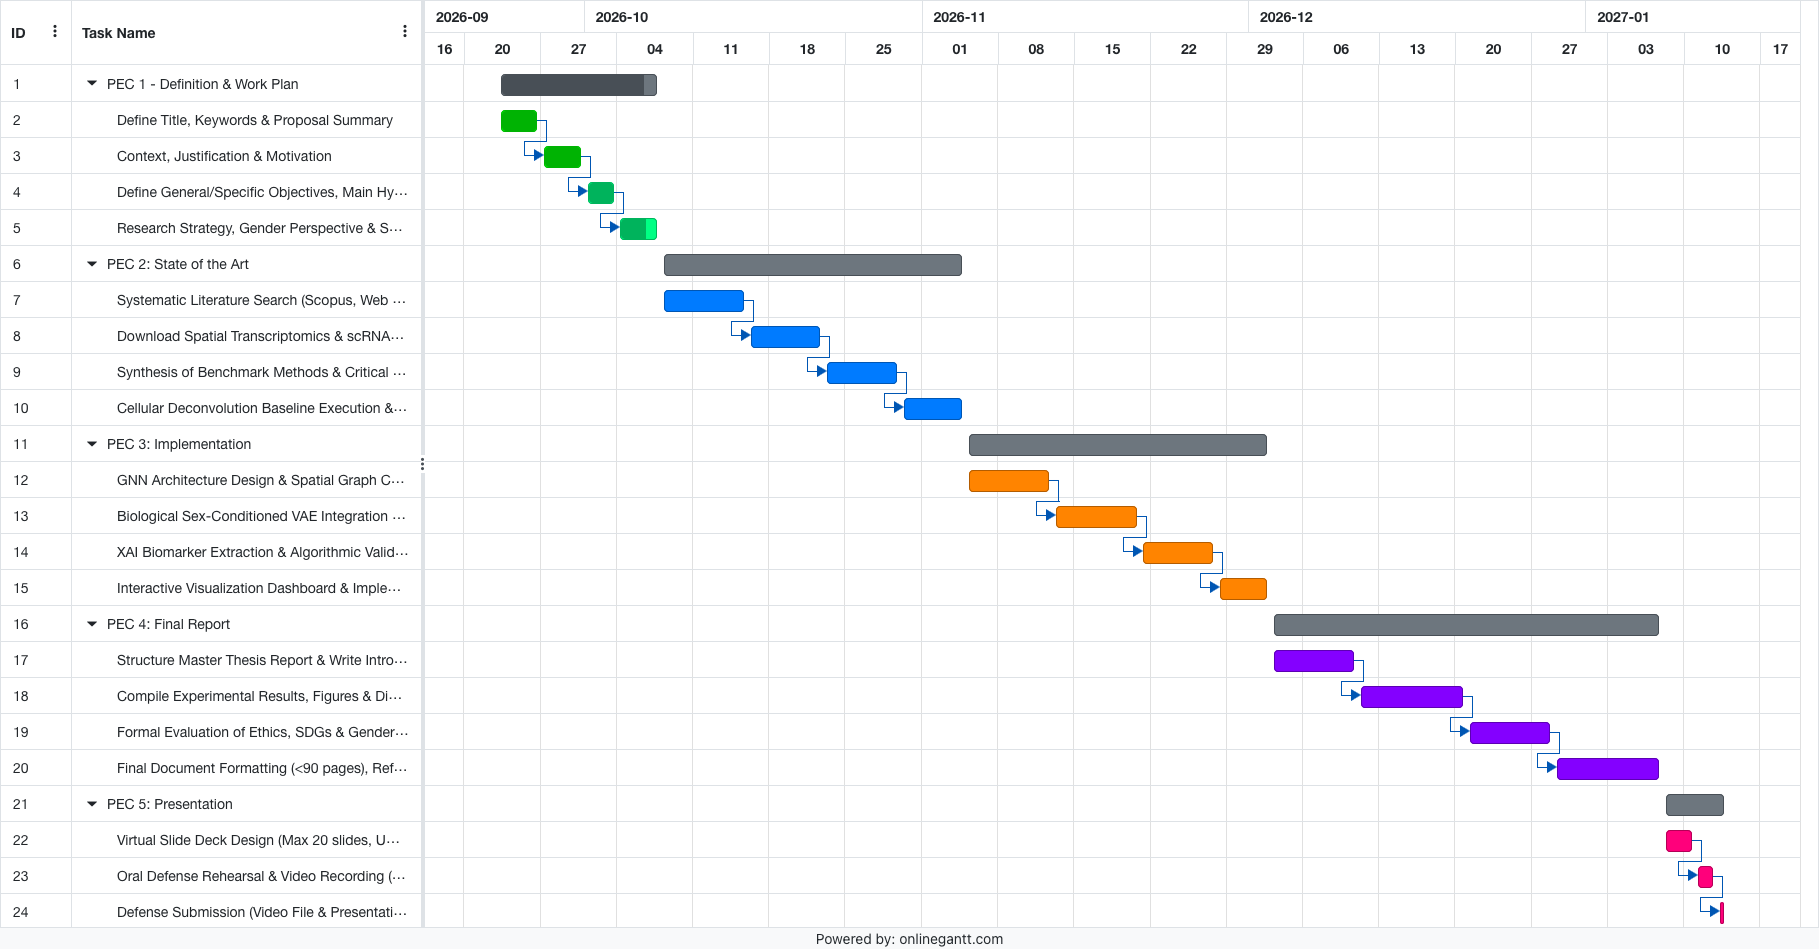
\includegraphics[width=0.9\linewidth]{Online Gantt 20261002.png}
    \caption{Master's Thesis Schedule and Work Breakdown Structure.}
    \label{fig:gantt_schedule}
\end{figure}
\end{landscape}


\begin{figure}[htbp]
\begin{center}

\end{center}
\end{figure}

%
%\newpage
%\chapter{PEC 2}

TBD

%\chapter{State of Art}

%State of the art of the subject in question. It should end up showing why work is important and contributes something, and with the hypotheses of work.

%
%\newpage
%\chapter{PEC3 - Example Statement on the use of generative artificial intelligence}

Explanation of any use made of generative artificial intelligence tools (such as ChatGPT, Gemini, DALL-E, or others) during the conception and development of this Final Project, as well as the writing of this report and the preparation of the presentation. It is mandatory to specify the concrete tools used, the purpose (e.g., ideation, code outlining, grammatical correction, image generation, etc.), the periods or phases of the work in which they were employed, the actions taken to validate the content generated by AI, and a critical evaluation of the impact of their use. It must be explicitly clarified which parts of the work are entirely the student's authorship and which have been based on inputs or results generated by AI, ensuring at all times that the intellectual responsibility and final validation of the content fall entirely upon the student, and that its use has been discussed with the Project supervisor and carried out in accordance with their instructions.


 
\textbf{Chapter structuring may vary depending on the type of work.}  
 
If applicable, a section on “Economic evaluation of work” will be included. This section will indicate the expenses associated with the development and maintenance of work, as well as the economic benefits obtained and a final analysis on the viability of the product.
%
%\newpage
%\chapter{PEC3 - Results}

Detail in this section the results obtained using the methodology described in the previous section.


%Recull of job results. There should be a correspondence with the methodology that the results are what is obtained after applying the methodology.

The figures must be explained and quoted in the text, such as \ref{fig:my_label}, in which the error is shown depending on the distance, in arbitrary units. All graphs must have the title of the axes.

\begin{figure}[!htbp]
    \centering
    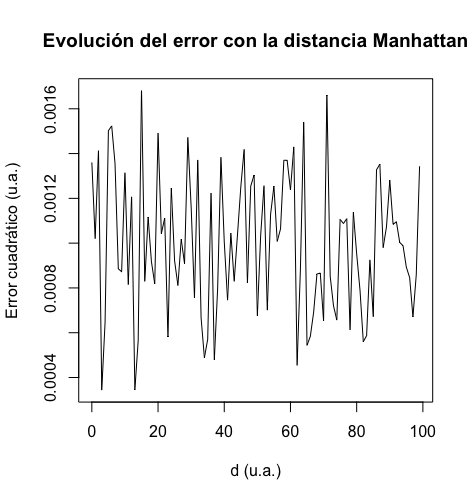
\includegraphics[width=7truecm]{Rplotmanh.png}
    \caption{Error working distance in arbitrary units.}
    \label{fig:my_label}
\end{figure}
%
%\newpage
%%\chapter{Discussion}
%Discussion of results in project context. It is in this section that they make sense and in which the research questions are answered and it is shown how the results respond to the problems raised.

%This part may not apply depending on the type of work.

%\chapter{Economic evaluation}
%If applicable, a section of ``Economic evaluation of work' will be included. This section will indicate the expenses associated with the development and maintenance of work, as well as the economic benefits obtained. A final analysis on the viability of the product must be carried out.

\chapter{PEC 3 - Conclusions and future works}

%\section{Conclusions}
This chapter must include:
\begin{itemize}
\item A description of the conclusions of the work:
\begin{itemize}
    \item Once the results have been obtained, what conclusions are drawn?
    \item Are these results as expected? Or have they been amazing? Why?
\end{itemize}
\item A critical reflection on the achievement of the objectives initially set:
\begin{itemize}
    \item Have we achieved all the objectives? If the answer is negative, why?
\end{itemize}
\item A critical analysis of the monitoring of planning and methodology throughout the product:
\begin{itemize}
    \item Has the schedule been followed?
    \item Has the planned methodology been adequate enough?
    \item Has it been necessary to introduce changes to ensure the success of the work? Why?
\end{itemize}
\item From the impacts foreseen in \ref{s:etic}, ethical-social, sustainability and diversity, evaluate/mention whether they have been mitigated (if they were negative) or whether they have been achieved (if they were positive). 
\item If unforeseen impacts have appeared in \ref{s:etic}, evaluate/mention how they have mitigated (if they were negative) or what they have contributed (if they were positive).
\item The future lines of work that have not been explored in this work and have remained pending.


%\item A description of the conclusions of the work: What lessons have been learned from work?
%\item A critical reflection on the achievement of the objectives initially set: Have we achieved all the objectives? If the answer is negative, why?
%\item Of the impacts foreseen in the section \ref{s:etic}, an assessment, or at least mention, of whether they have been mitigated (if they were negative) or whether they have been achieved (if they were positive). 
\end{itemize}

%\section{Future Lines}
%The future lines of work that could not be explored in this work and have been pending.

%\section{Schedule Tracking}
%A critical analysis of the monitoring of the planning and methodology throughout the work: 
%\begin{itemize}
%    \item  Have the schedule been followed? 
%    \item Has the planned methodology been adequate? 
%    \item Has it been necessary to introduce changes to ensure the success of the work? Why?
%\end{itemize}

%
%\newpage
%\chapter{Glossary}

Definition of the most relevant terms and acronyms used in the Report.

%Defining the most relevant terms and acronyms used within the Memory.

\chapter{Bibliography}

Numbered list of bibliographic references used within memory. In each place where a reference is used within the text, it must be indicated by quoting the reference number, for example: [7].

It is very important to include all the references used and quote them appropriately, that is, including all the information necessary to identify the reference. The minimum information to be included according to the reference type is:

\begin{itemize}
\item Book: Authors, Title, Edition (if applicable) Editorial, City, Year.
\item  Journal article: Authors, Title, Name of the Journal, Home and End Page Number, Issue of the magazine / Volume, Year.
\item  Web: URL and date it was visited.
\end{itemize}

Information on how to quote documents: \url{http://biblioteca.uoc.edu/es/recursos/citacion-bibliografica}.
%

\newpage
% ============================================================
% Multimodal Integration Spatial Transcriptomics ? TFM Bibliography
% MU Bioinformatics i Bioestad�stics � UOC/UB � 2025-2026
% Format: thebibliography ? APA 7th edition
% Author: Marco Russo
% Note: also available as references.bib for BibTeX workflows
% ============================================================


\begin{thebibliography}{99}
 
% ?? Cardiovascular sex differences ?????????????????????????
 
\bibitem{hartman2023sex}
Hartman, R. J. G., et al. (2023).
Sex differences in the genetic and molecular mechanisms of coronary artery disease.
\textit{Atherosclerosis}, \textit{384}, 117434.
\url{https://doi.org/10.1016/j.atherosclerosis.2023.117434}
 
\bibitem{reif2025consideration}
Reif, A., et al. (2025).
Consideration of sex/gender aspects in cardiovascular clinical trials.
\textit{BMC Cardiovascular Disorders}, \textit{25}, 471.
\url{https://doi.org/10.1186/s12872-025-04714-8}
 
\bibitem{sukhavasi2025single}
Sukhavasi, K., et al. (2025).
Single-cell RNA sequencing reveals sex differences in subcellular composition of human carotid plaques.
\textit{Nature Cardiovascular Research}, \textit{4}, 412--432.
\url{https://doi.org/10.1038/s44161-025-00628-y}
 
% ?? Spatial transcriptomics (cardiovascular) ???????????????
 
\bibitem{kanemaru2023spatially}
Kanemaru, K., et al. (2023).
Spatially resolved multiomics of human cardiac niches.
\textit{Nature}, \textit{619}(7971), 801--810.
\url{https://doi.org/10.1038/s41586-023-06311-1}
 
\bibitem{campos2025spatial}
Campos, J., et al. (2025).
Spatial transcriptomics elucidates localized immune responses in atherosclerotic coronary artery.
\textit{EMBO Molecular Medicine}, \textit{17}(10), 2827--2846.
\url{https://doi.org/10.1038/s44321-025-00280-w}
 
\bibitem{slenders2024single}
Slenders, L., et al. (2024).
Single cell spatial transcriptomics integration deciphers morphological heterogeneity of atherosclerotic carotid arteries.
\textit{Nature Communications}, \textit{15}, 6767.
\url{https://doi.org/10.1038/s41467-025-67679-4}
 
% ?? GNN methods for spatial transcriptomics ????????????????
 
\bibitem{hu2021spagcn}
Hu, J., et al. (2021).
SpaGCN: Integrating gene expression, spatial location and histology to identify spatial domains and spatially variable genes by graph convolutional network.
\textit{Nature Methods}, \textit{18}(11), 1342--1351.
\url{https://doi.org/10.1038/s41592-021-01255-8}
 
\bibitem{dong2022deciphering}
Dong, K., \& Zhang, S. (2022).
Deciphering spatial domains from spatially resolved transcriptomics with an adaptive graph attention auto-encoder.
\textit{Nature Communications}, \textit{13}, 1739.
\url{https://doi.org/10.1038/s41467-022-29439-6}
 
\bibitem{long2023spatially}
Long, Y., et al. (2023).
Spatially informed clustering, integration, and deconvolution of spatial transcriptomics with GraphST.
\textit{Nature Methods}, \textit{20}(7), 1053--1063.
\url{https://doi.org/10.1038/s41592-023-01809-8}
 
% ?? Deep Learning foundations ??????????????????????????????
 
\bibitem{kipf2016variational}
Kipf, T. N., \& Welling, M. (2016).
Variational Graph Auto-Encoders.
\textit{arXiv preprint arXiv:1611.07308}.
\url{https://arxiv.org/abs/1611.07308}
 
\bibitem{velickovic2018graph}
Veli\v{c}kovi\'{c}, P., et al. (2018).
Graph Attention Networks.
\textit{International Conference on Learning Representations (ICLR)}.
\url{https://arxiv.org/abs/1710.10903}
 
\bibitem{bronstein2021geometric}
Bronstein, M. M., et al. (2021).
Geometric Deep Learning: Grids, Groups, Graphs, Geodesics, and Gauges.
\textit{arXiv preprint arXiv:2104.13478}.
\url{https://arxiv.org/abs/2104.13478}
 
% ?? Multi-omics integration ????????????????????????????????
 
\bibitem{argelaguet2020mofa}
Argelaguet, R., et al. (2020).
MOFA+: a statistical framework for comprehensive integration of multi-modal single-cell data.
\textit{Genome Biology}, \textit{21}(1), 111.
\url{https://doi.org/10.1186/s13059-020-02015-1}
 
\bibitem{losert2024multiomic}
Losert, C., et al. (2024).
Multiomic analyses uncover immunological signatures in acute and chronic coronary syndromes.
\textit{Nature Medicine}, \textit{30}, 2953--2964.
\url{https://doi.org/10.1038/s41591-024-02953-4}
 
% ?? Deconvolution ??????????????????????????????????????????
 
\bibitem{elosua2021spotlight}
Elosua-Bayes, M., et al. (2021).
SPOTlight: seeded NMF regression to deconvolute spatial transcriptomics spots with single-cell transcriptomes.
\textit{Nucleic Acids Research}, \textit{49}(9), e50.
\url{https://doi.org/10.1093/nar/gkab043}
 
% ?? Ethics and gender equity ???????????????????????????????
 
\bibitem{heidari2016sex}
Heidari, S., et al. (2016).
Sex and Gender Equity in Research: rationale for the SAGER guidelines and recommended use.
\textit{Research Integrity and Peer Review}, \textit{1}(1), 2.
\url{https://doi.org/10.1186/s41073-016-0007-6}
 
\end{thebibliography}


\newpage
\appendix


List of sections that are too extensive to include in memory and have a self-contained character (e.g. user manuals, installation manuals, etc.)
 
Depending on the type of work, there may be no need to add an annex.



\end{document}
